% Compact PGFPlots panel for the surface5 BSC bit-scale decomposition.
% Requires \usepackage{pgfplots} and \pgfplotsset{compat=1.18}.
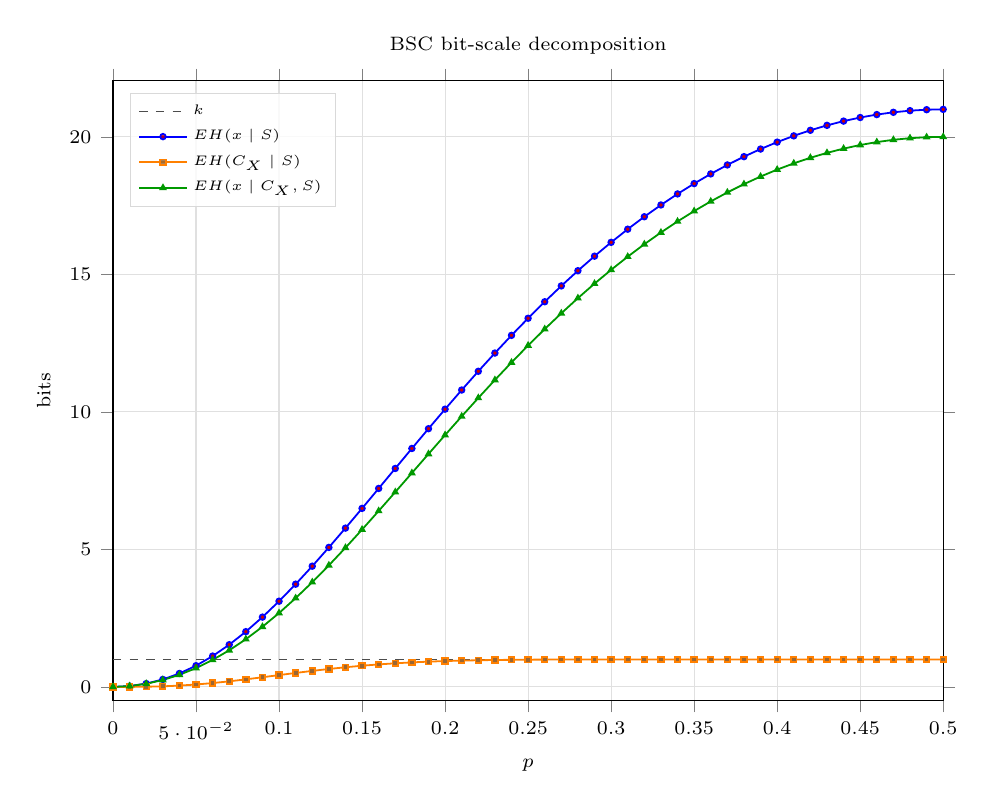
\begin{tikzpicture}
\begin{axis}[
  name=surfaceFiveBSCBitScaleAxis,
  width=\linewidth,
  height=0.78\linewidth,
  title={BSC bit-scale decomposition},
  title style={font=\scriptsize},
  xlabel={$p$},
  ylabel={bits},
  xmin=0, xmax=0.5,
  ymin=-0.5, ymax=22.05,
  grid=both,
  major grid style={black!12},
  minor grid style={black!6},
  tick align=outside,
  tick label style={font=\scriptsize},
  label style={font=\scriptsize},
  legend cell align={left},
  legend style={draw=black!15, fill=white, fill opacity=0.82, text opacity=1, at={(0.02,0.98)}, anchor=north west, font=\tiny},
]
\addplot[black!70, dashed, line width=0.55pt] coordinates {(0,1) (0.5,1)};
\addlegendentry{$k$}
\addplot+[color=blue, mark=*, mark size=1.0pt, line width=0.65pt]
coordinates {(0,0) (0.01,0.0309769830461) (0.02,0.120831945811) (0.03,0.272361948826) (0.04,0.488797485428) (0.05,0.771876603271) (0.06,1.12138210074) (0.07,1.53513383979) (0.08,2.00921740614) (0.09,2.53833335165) (0.1,3.11619011785) (0.11,3.73588882484) (0.12,4.39026752796) (0.13,5.07218771739) (0.14,5.77475710997) (0.15,6.49149052908) (0.16,7.21641542739) (0.17,7.94413101518) (0.18,8.66983065584) (0.19,9.38929675608) (0.2,10.0988762848) (0.21,10.7954436608) (0.22,11.4763563061) (0.23,12.1394068298) (0.24,12.7827746676) (0.25,13.4049790888) (0.26,14.0048347886) (0.27,14.5814107721) (0.28,15.1339928838) (0.29,15.6620500896) (0.3,16.1652044549) (0.31,16.6432046576) (0.32,17.0959028062) (0.33,17.5232342982) (0.34,17.9252004376) (0.35,18.3018535266) (0.36,18.6532841579) (0.37,18.9796104469) (0.38,19.2809689634) (0.39,19.5575071428) (0.4,19.8093769779) (0.41,20.0367298149) (0.42,20.2397120932) (0.43,20.4184618923) (0.44,20.5731061599) (0.45,20.7037585141) (0.46,20.8105175262) (0.47,20.8934654027) (0.48,20.9526669995) (0.49,20.9881691122) (0.5,21)};
\addlegendentry{$\mathbb{E}H(x\mid S)$}
\addplot+[color=orange, mark=square*, mark size=1.0pt, line width=0.65pt]
coordinates {(0,0) (0.01,0.000853674247968) (0.02,0.00660709261872) (0.03,0.0214113132062) (0.04,0.048071359864) (0.05,0.0877491333268) (0.06,0.14002193905) (0.07,0.203174747096) (0.08,0.274607361009) (0.09,0.351261836865) (0.1,0.43000529969) (0.11,0.507931588993) (0.12,0.582568205144) (0.13,0.651991518033) (0.14,0.714863375384) (0.15,0.770407168315) (0.16,0.818342437036) (0.17,0.858795564465) (0.18,0.89220114361) (0.19,0.919205080745) (0.2,0.94057700689) (0.21,0.957136478236) (0.22,0.969694931964) (0.23,0.979013476262) (0.24,0.985775294932) (0.25,0.990570652886) (0.26,0.993892094798) (0.27,0.996137332654) (0.28,0.997617430782) (0.29,0.998568150495) (0.3,0.999162660096) (0.31,0.999524210878) (0.32,0.999737791171) (0.33,0.999860164439) (0.34,0.999928040662) (0.35,0.999964397021) (0.36,0.999983141502) (0.37,0.999992404846) (0.38,0.999996768766) (0.39,0.99999871448) (0.4,0.999999527815) (0.41,0.999999842584) (0.42,0.999999953468) (0.43,0.9999999882) (0.44,0.999999997554) (0.45,0.999999999616) (0.46,0.99999999996) (0.47,0.999999999998) (0.48,1) (0.49,1) (0.5,1)};
\addlegendentry{$\mathbb{E}H(C_X\mid S)$}
\addplot+[color=green!60!black, mark=triangle*, mark size=1.0pt, line width=0.65pt]
coordinates {(0,0) (0.01,0.0301233087981) (0.02,0.114224853192) (0.03,0.25095063562) (0.04,0.440726125564) (0.05,0.684127469945) (0.06,0.981360161694) (0.07,1.33195909269) (0.08,1.73461004513) (0.09,2.18707151478) (0.1,2.68618481816) (0.11,3.22795723585) (0.12,3.80769932281) (0.13,4.42019619936) (0.14,5.05989373459) (0.15,5.72108336076) (0.16,6.39807299035) (0.17,7.08533545071) (0.18,7.77762951223) (0.19,8.47009167534) (0.2,9.15829927793) (0.21,9.83830718256) (0.22,10.5066613741) (0.23,11.1603933536) (0.24,11.7969993726) (0.25,12.4144084359) (0.26,13.0109426938) (0.27,13.5852734395) (0.28,14.1363754531) (0.29,14.6634819391) (0.3,15.1660417948) (0.31,15.6436804468) (0.32,16.096165015) (0.33,16.5233741337) (0.34,16.9252723969) (0.35,17.3018891296) (0.36,17.6533010164) (0.37,17.9796180421) (0.38,18.2809721946) (0.39,18.5575084283) (0.4,18.8093774501) (0.41,19.0367299723) (0.42,19.2397121397) (0.43,19.4184619041) (0.44,19.5731061624) (0.45,19.7037585145) (0.46,19.8105175262) (0.47,19.8934654027) (0.48,19.9526669995) (0.49,19.9881691122) (0.5,20)};
\addlegendentry{$\mathbb{E}H(x\mid C_X,S)$}
\end{axis}
\end{tikzpicture}
